\documentclass[style=simple]{powerdot}
\usepackage[utf8]{inputenc}
\usepackage{wrapfig}
\usepackage{hyperref}
%\title{Stealthy Malware Traffic --- Not as Innocent as It Looks}
%\author{Xingsi Zhong, Yu Fu, Lu Yu, Richard R. Brooks and G. Kumar Venayagamoorthy}
%\date{October, 2015}
%\hypersetup{pdfpagemode=Landscape}
\usepackage{graphicx} 
\pdsetup{
  logohook=t,
  logopos={.90\slidewidth,.99\slideheight},
  logocmd={
\includegraphics[height=0.2in]{./wordmark-academic.eps}},
}

\title{Security of Distributed Cyber-Physical Systems with Connected Vehicle Applications} 
%\author{Xingsi Zhong, Yu Fu, Lu Yu, Richard R. Brooks \\ \qquad\quad and G. Kumar Venayagamoorthy, \\ Clemson University}
\author{PI : Dr. Pierluigi Pisu\\Automotive Engineering Department (CUICAR)\\
Co-PI : Dr. Richard Brooks\\Electrical and Computer Engineering Department\\
Co-PI : Dr. Jim Martin \\School of Computing \\
Clemson University 
\\
%Acknowledgement: U.S. National Science Foundation, under Grant IIP \# 1312260.
}


\begin{document}
\maketitle				% OPTIONAL
\section[tocsection=false,slide=false]{Outline}
\begin{slide}{OUTLINE}
\textcolor{blue}{} \\
\textcolor{blue}{} \\
  \begin{itemize}
\item Overview
\item Motivation \& Introduction
\item Problem Statement
\item Scenario I 
\begin{itemize}
\small
\item Hybrid modeling 
\item Detection
\normalsize
\end{itemize}
\item Scenario II
\begin{itemize}
\small
\item Game Theory : Attack Resilient Countermeasure
\normalsize
\end{itemize}
\item Experimental Setup 
\end{itemize}
\end{slide}

\section[tocsection=true,slide=false]{I. Overview}
\begin{slide}{Overview}
\begin{picture}(0,0)
   \put(0,-180){
     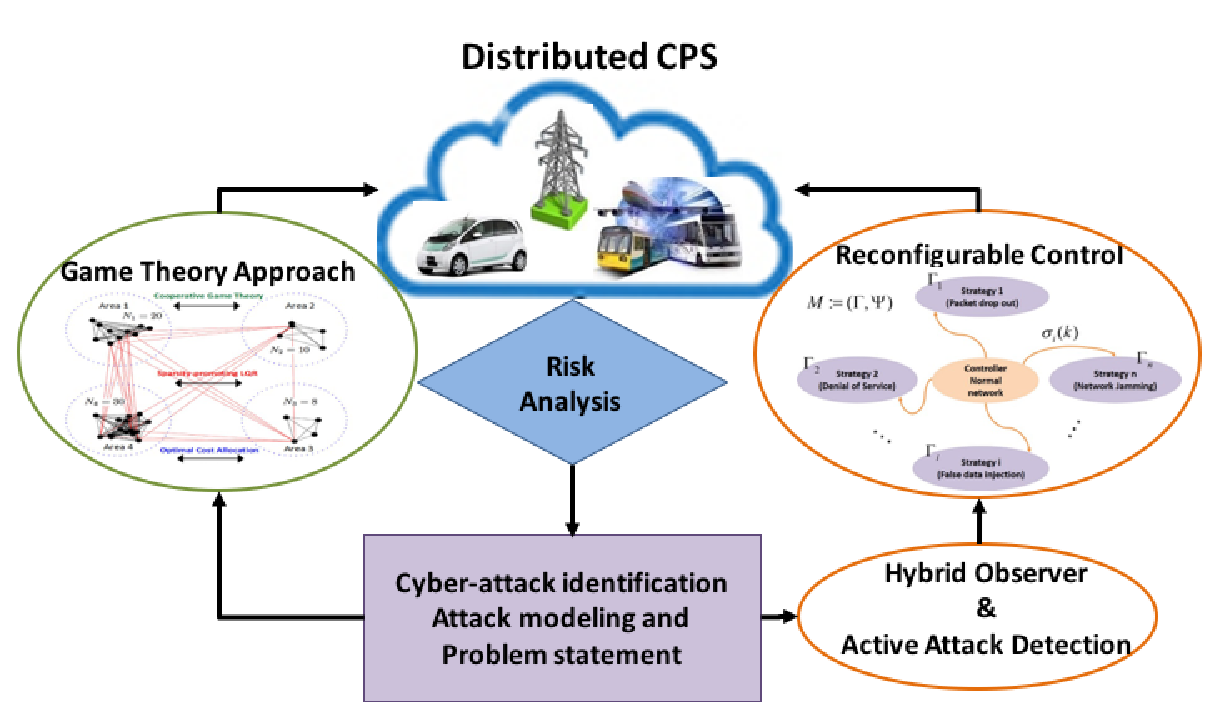
\includegraphics[width=4.2in]{DistributedCPS.eps}
     }
 \end{picture}
\end{slide}

\section[tocsection=true,slide=false]{II. Motivation \& Introduction}
\begin{slide}{Motivation}
\begin{itemize}
\item Intrusion detection systems (IDS) have shown their inability to detect and distinguish cyber-attacks from failures when CPS is concerned.
\item Damages to the vehicles in connected vehicles include but not limited to 
\begin{itemize}
\small 
\item False data injection to hamper system performance (energy or fuel efficient driving)
\item Collision between vehicles
\normalsize
\end{itemize}
\item The cyber security vulnerabilities that are associated with connected vehicles involve a number of parties: the vehicle users, the vehicle manufacturer, the suppliers, the insurance companies, public agencies and effectively anyone connected in the transportation network.
\end{itemize}
\end{slide}

\begin{slide}{Motivation}
\begin{itemize}
\item Cyber Physical System (CPS)
\begin{itemize}
\small 
\item Physical plant
\begin{itemize}
\small 
\item Multi agents/ Interconnected system 
\item Sensors / Actuators 
\normalsize
\end{itemize}
\item Communication network
\begin{itemize}
\small 
\item Global
\item Local 
\normalsize
\end{itemize}
\normalsize
\end{itemize}
\item Cyber-attacks
\begin{itemize}
\small 
\item Receiving information 
\item Sending data
\item Control process
\normalsize
\end{itemize}
\item Physical failure 
\begin{itemize}
\small 
\item Sensors / Actuators
\normalsize
\end{itemize}
\end{itemize}
\end{slide}

\section[tocsection=true,slide=false]{III. Problem Statements}
\begin{slide}{Cyber attacks on individual subsystem}
\begin{picture}(0,0)
   \put(40,-120){
     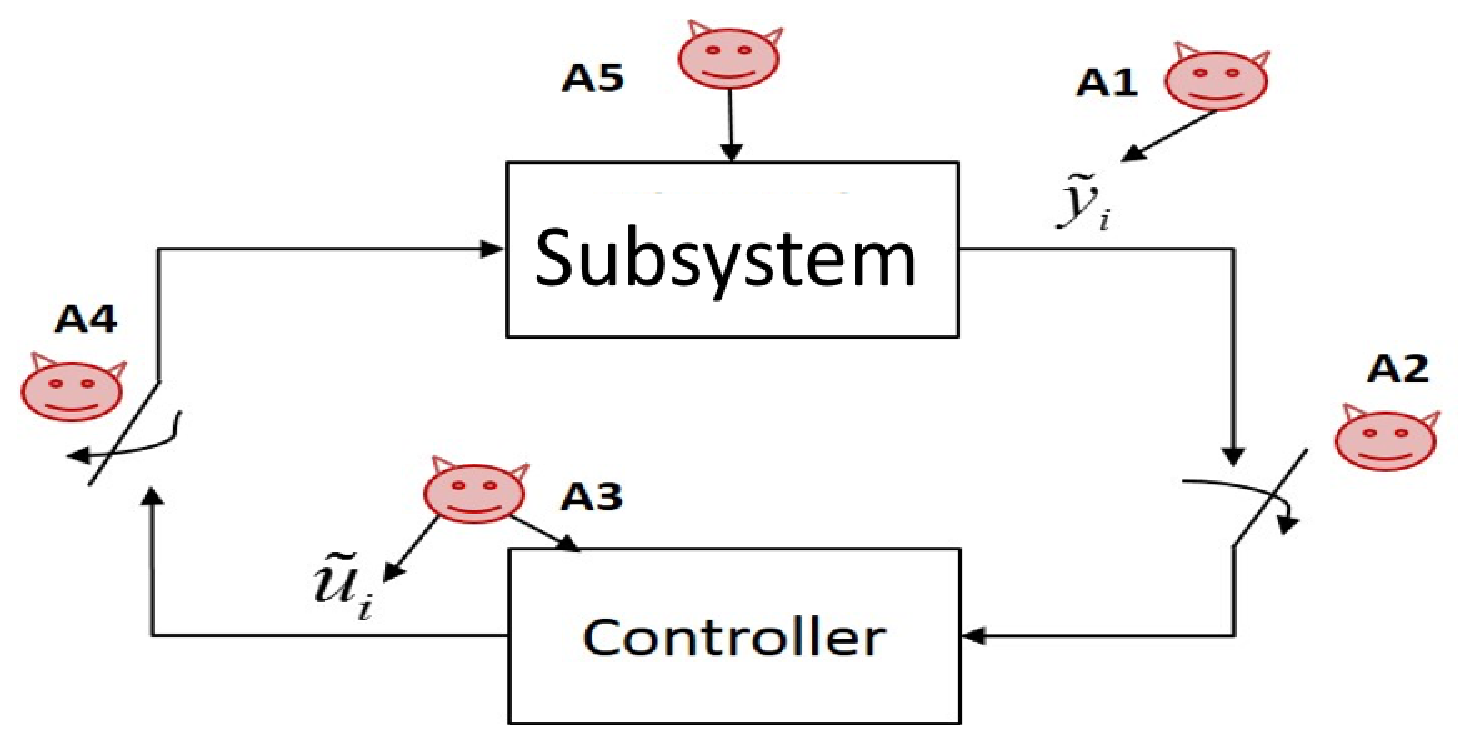
\includegraphics[width=3in]{subsys.eps}
     }
 \end{picture}
\end{slide}

\begin{slide}{Compromised subsystem in a distributed CPS}
\begin{picture}(0,0)
   \put(20,-190){
     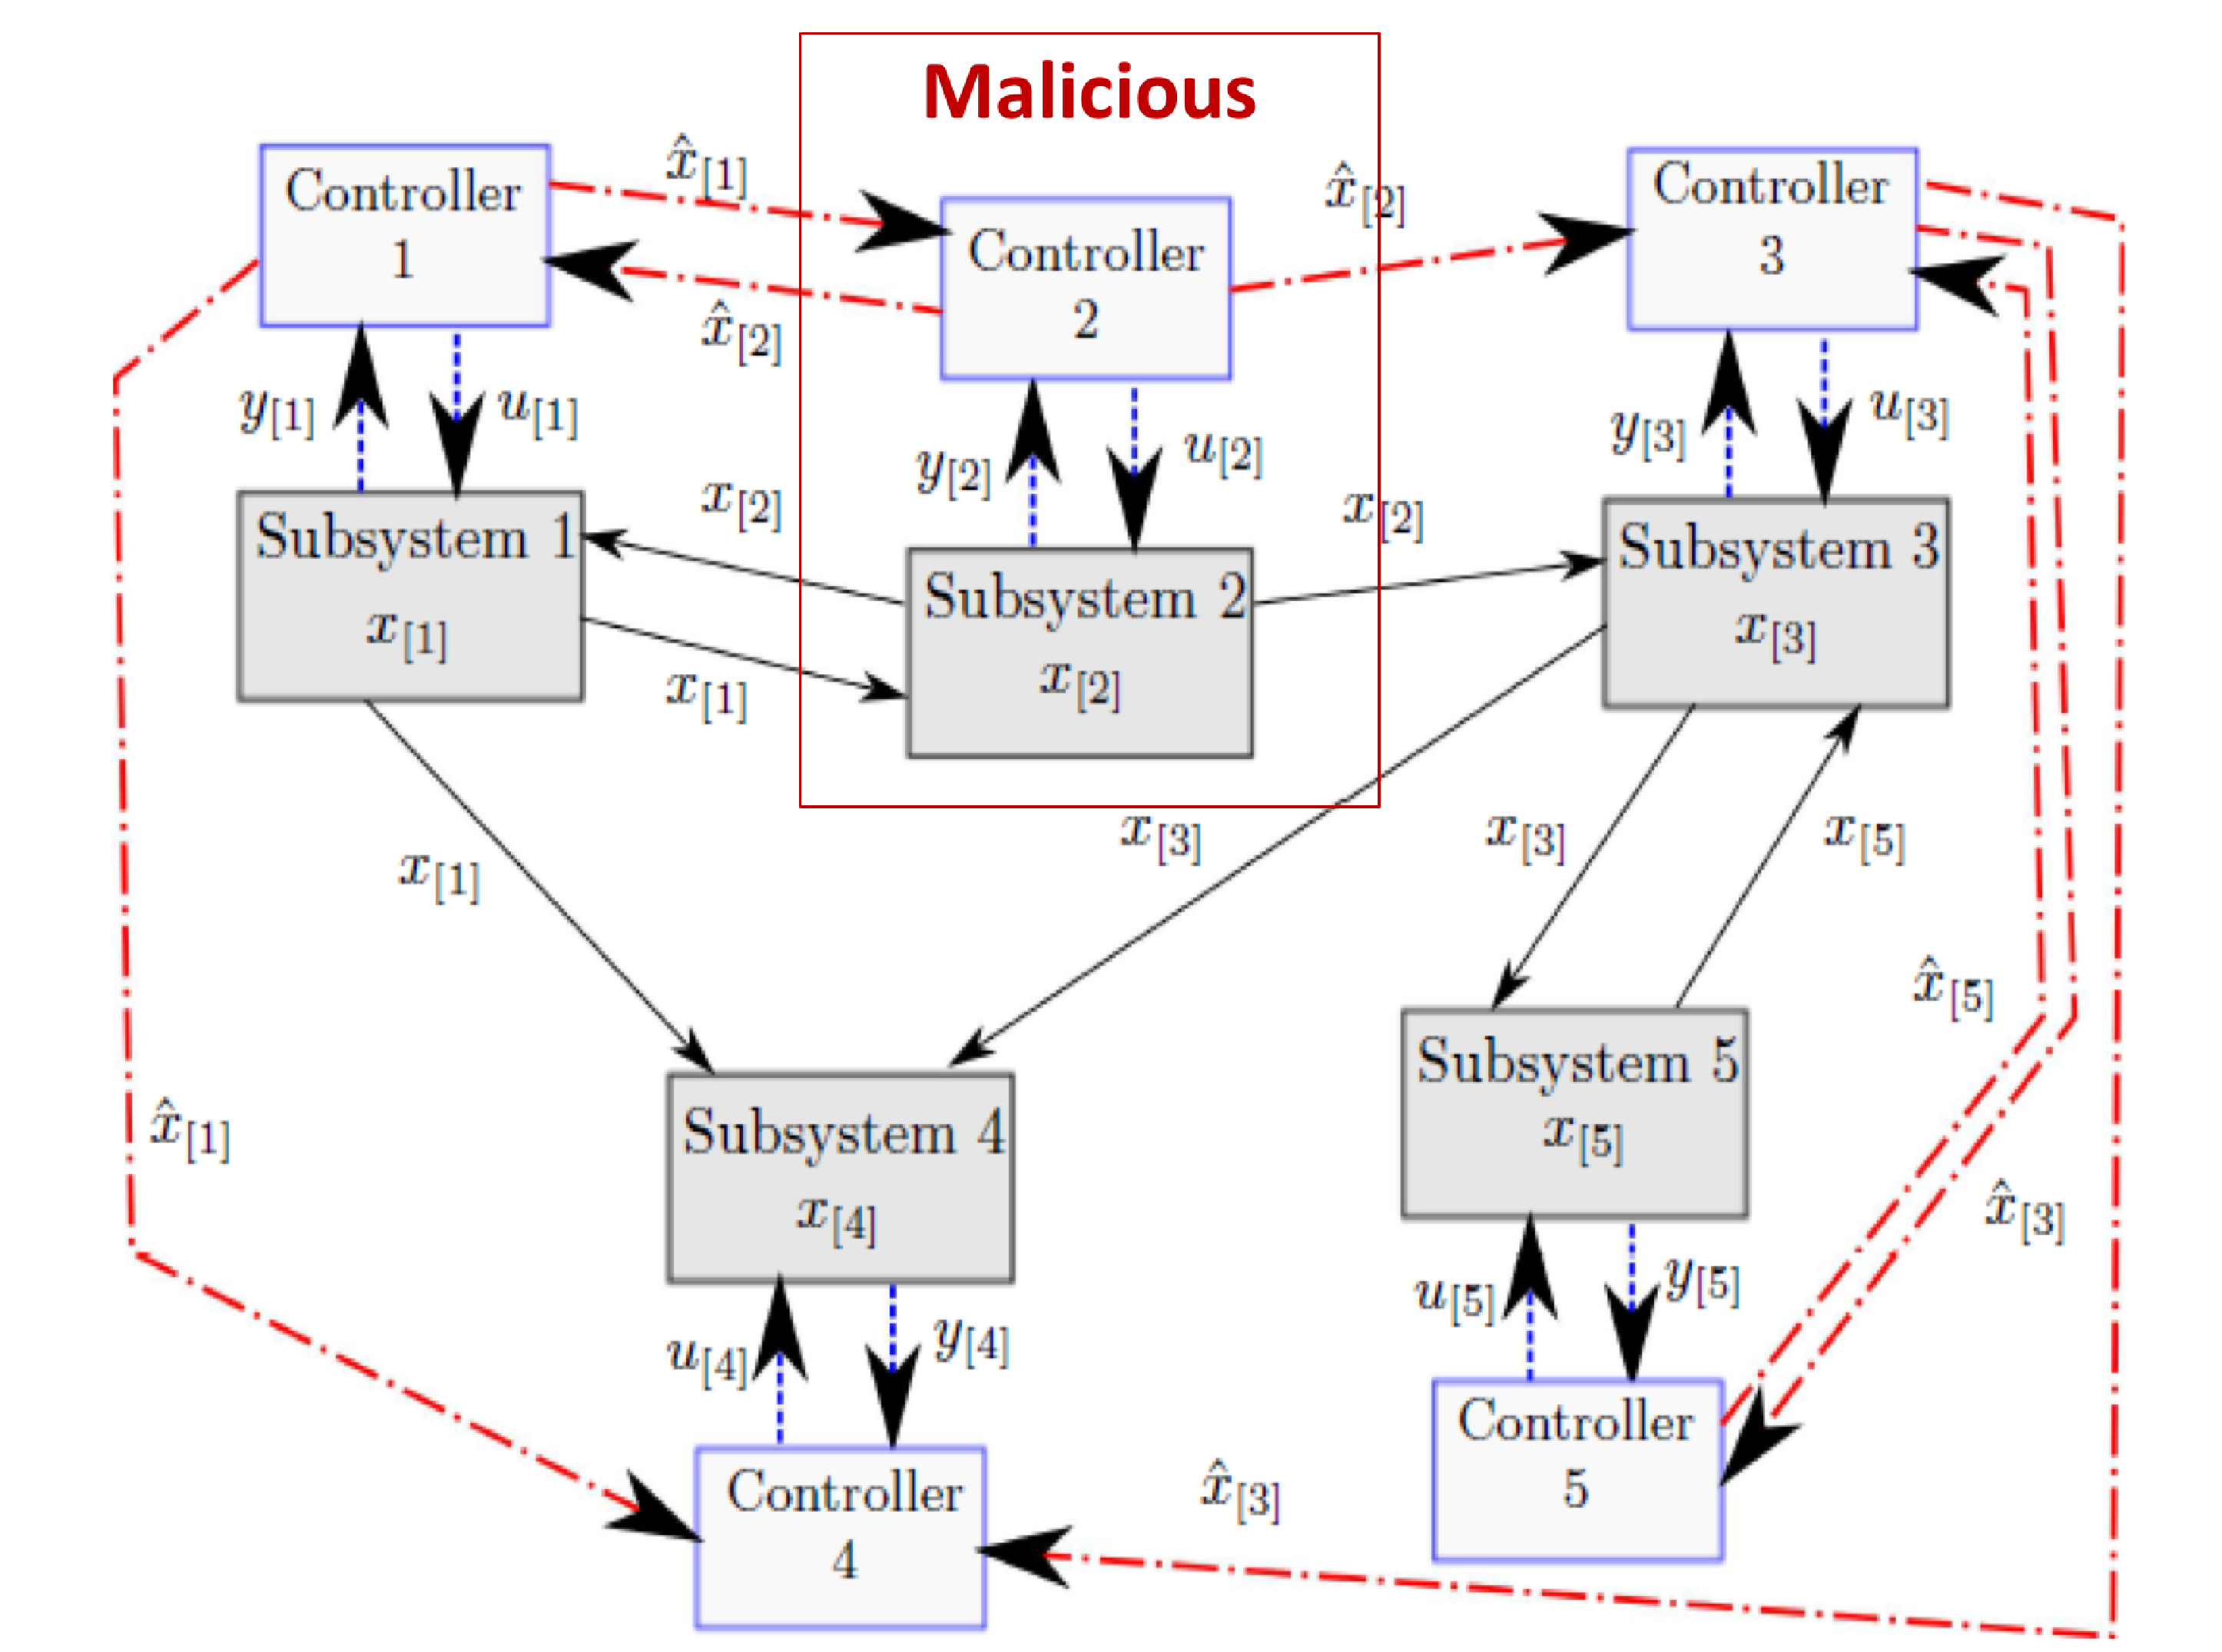
\includegraphics[width=3.4in]{compromised.eps}
     }
 \end{picture}
\end{slide}


\section[tocsection=true,slide=false]{IV. Scenario I}
\begin{slide}{Cyber attacks on individual subsystem}
\begin{picture}(0,0)
   \put(15,-160){
     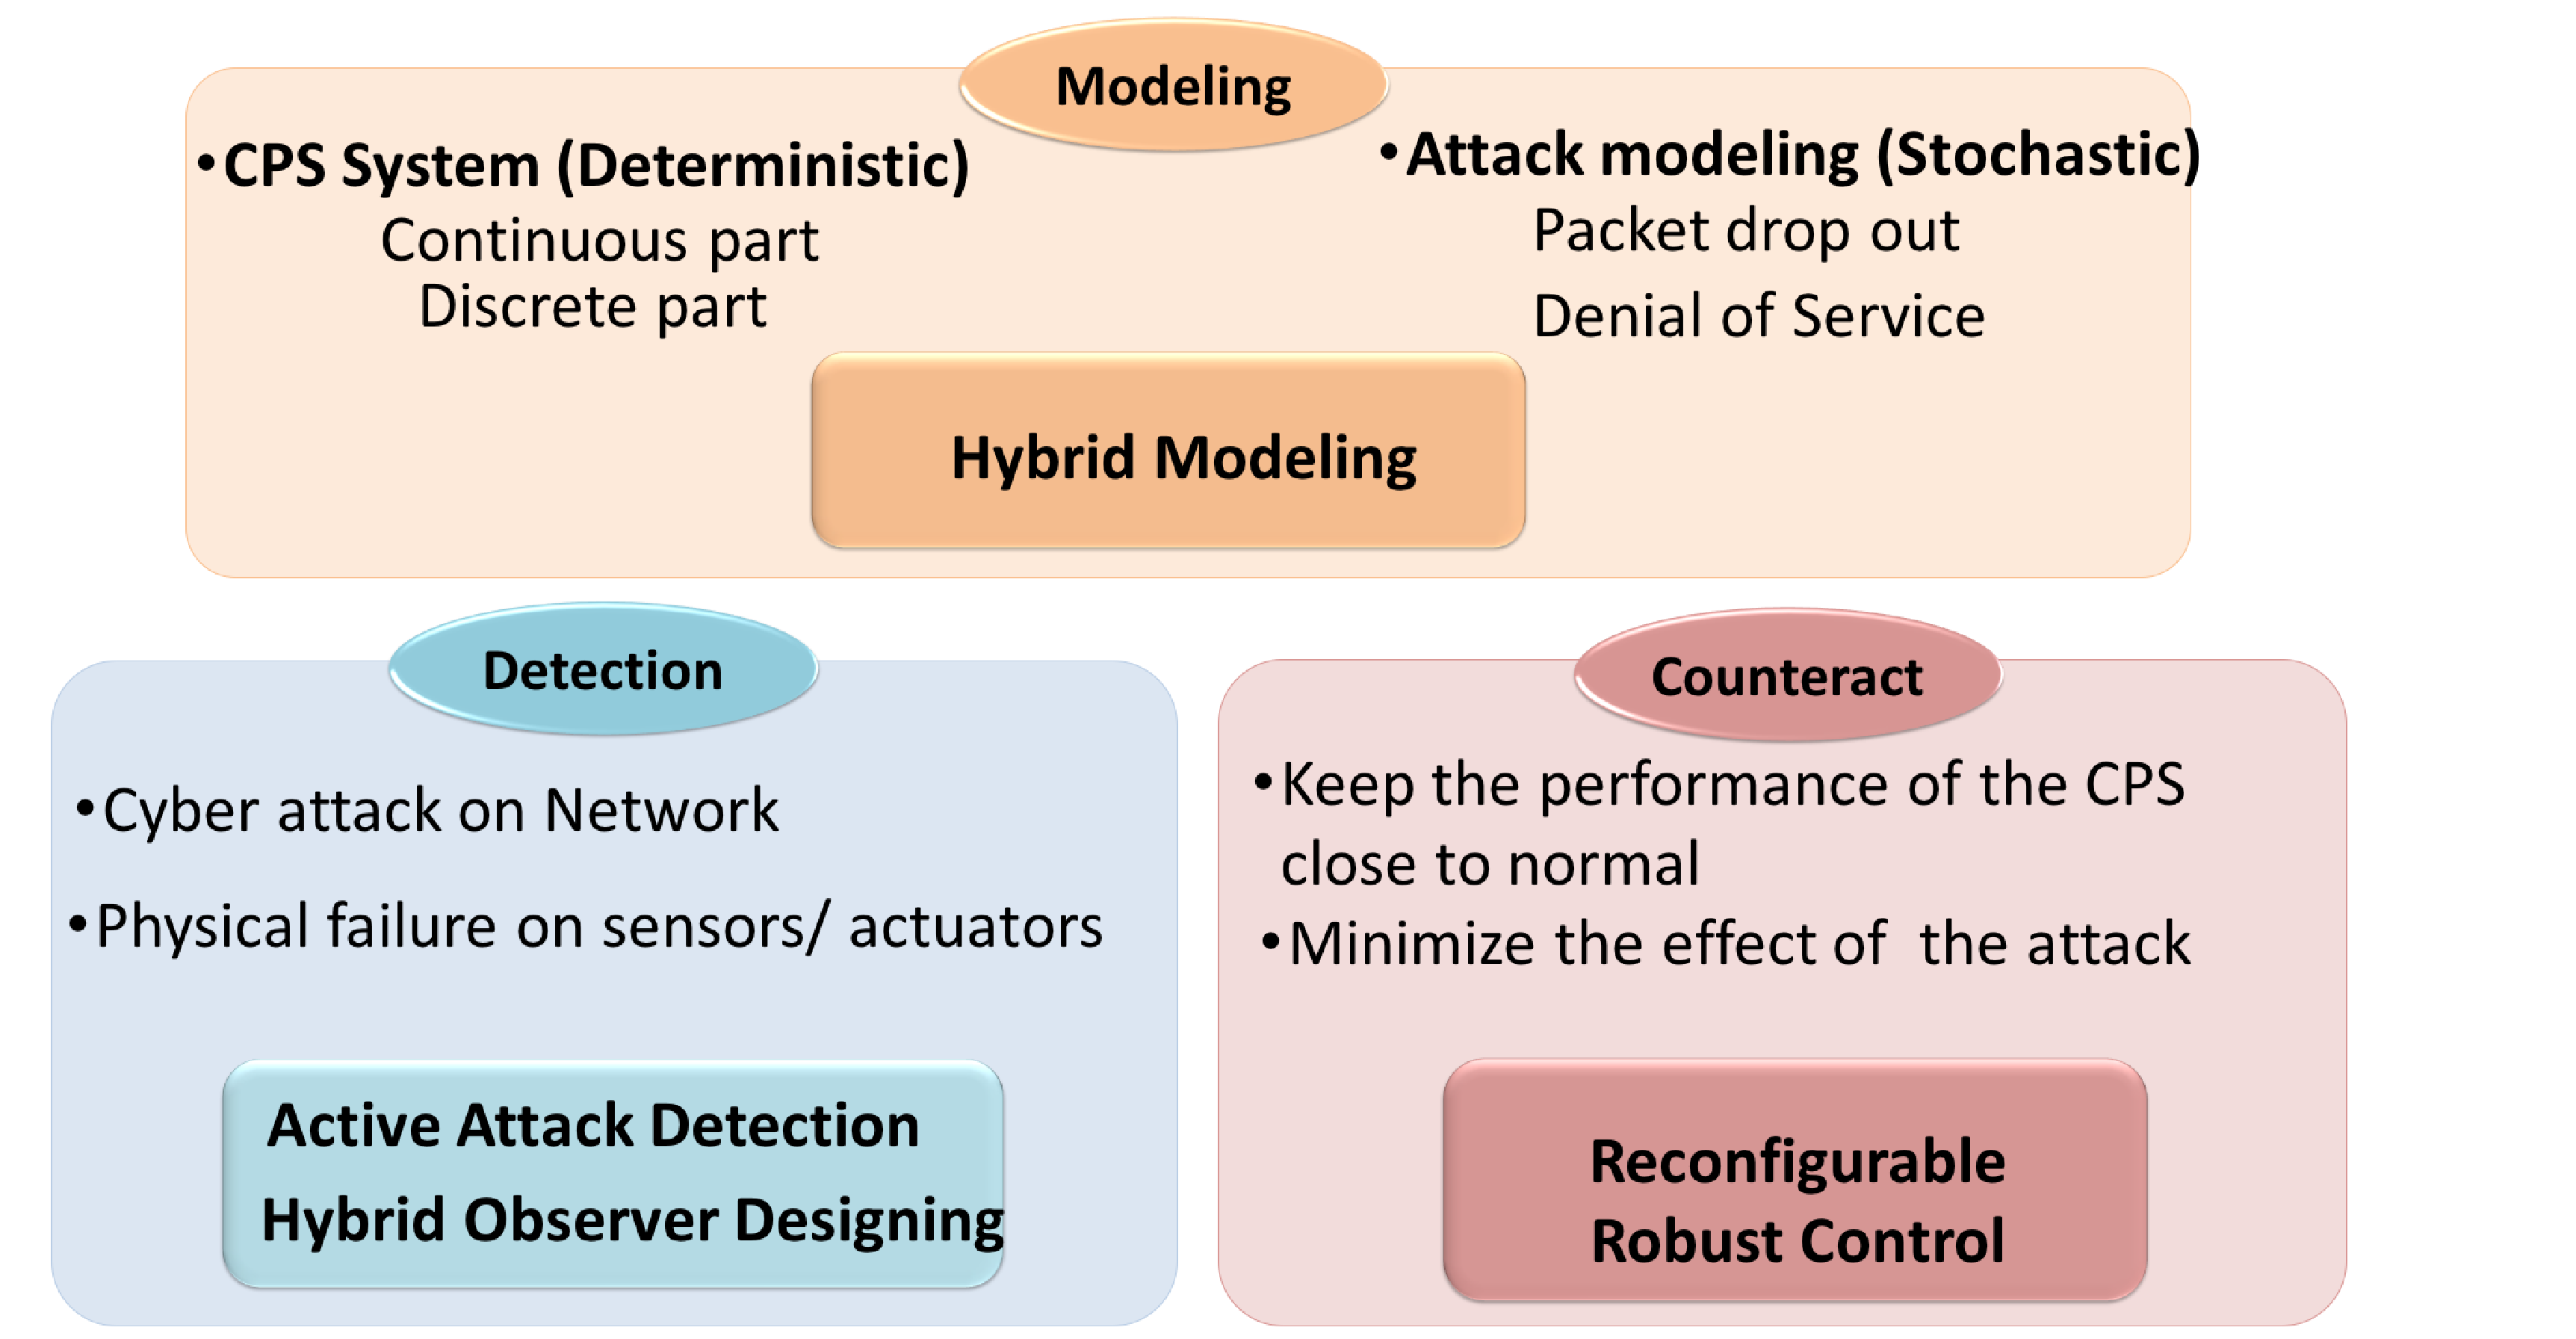
\includegraphics[width=4.2in]{S1.eps}
     }
 \end{picture}
\end{slide}

\begin{slide}{Hybrid Modeling and Control}
\begin{picture}(0,0)
   \put(130,-200){
     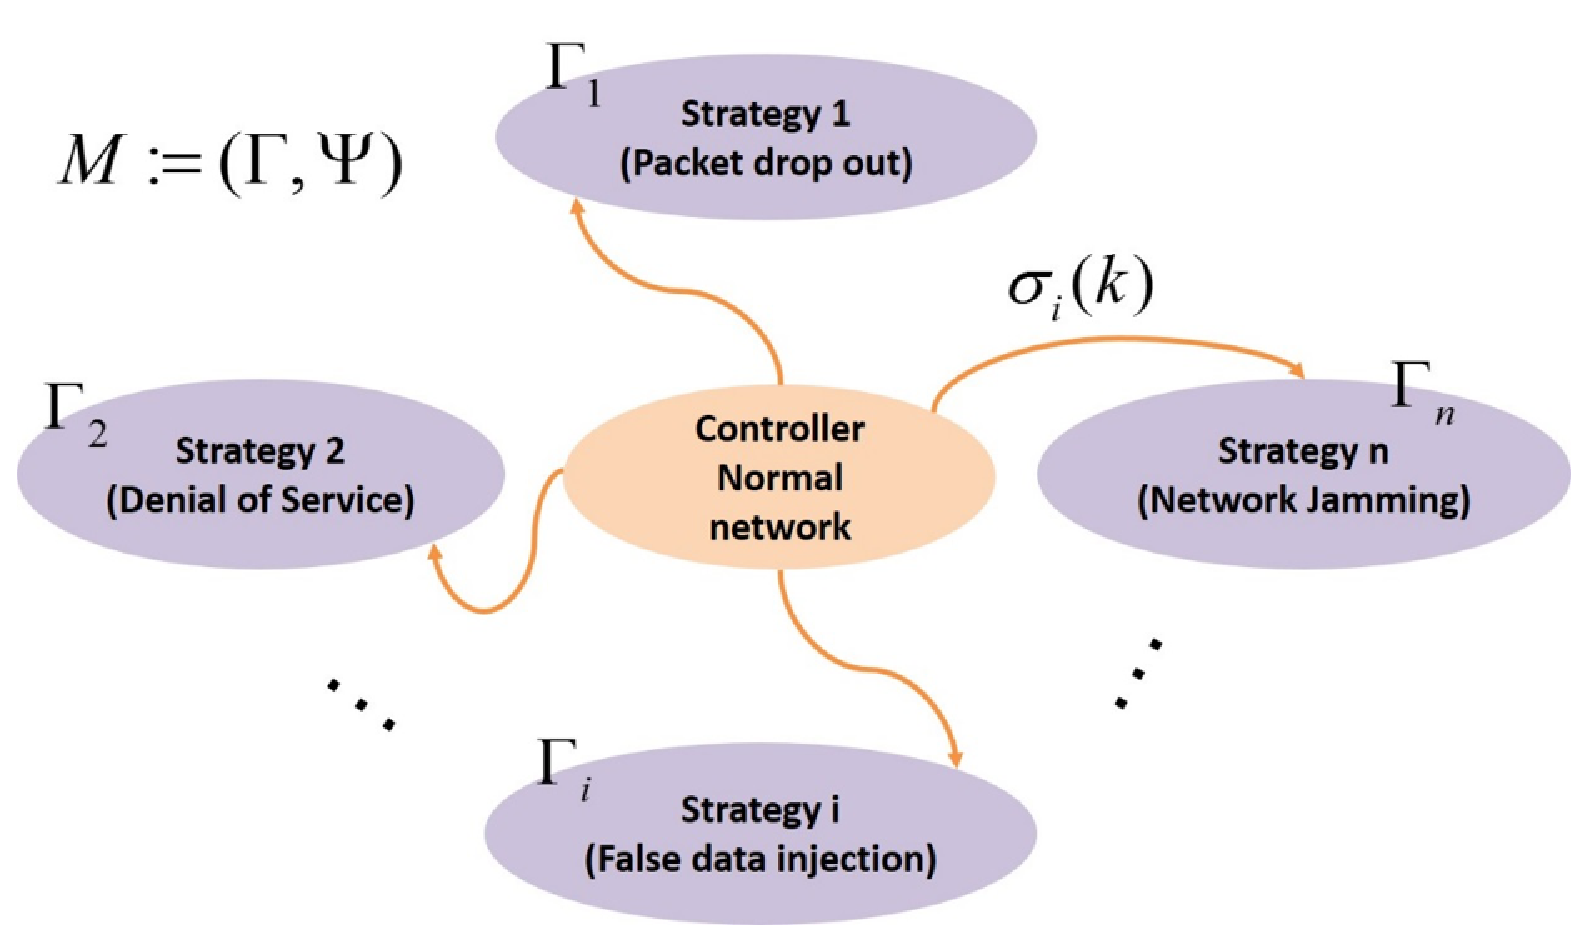
\includegraphics[width=2.5in]{S2.eps}
     }
 \end{picture}
\begin{itemize}
\item Hybrid system
\begin{itemize}
\small 
\item Different strategy for different cyber-attacks
\item Switch between strategies based on detection decision
\item $M$: Hybrid system
\item $\Gamma$: Set of discrete states of M
\item $\Psi$: Continuous dynamics of M
\item $\sigma(k)$ : Event
\normalsize
 \end{itemize}
 \item Assumptions 
\begin{itemize}
\small 
\item Continuous sub-systems:\\ LTI systems 
\normalsize
 \end{itemize}
 \end{itemize}
\end{slide}


\begin{slide}{Detection}
\begin{itemize}
\item Hybrid Observer 
\begin{itemize}
\small 
\item Considers the cyber and physical states of the CPS 
\item Makes decisions on cyber-attack by monitoring the augmented system
\item Has the potential to detect a wider range of cyber-attacks that includes common attacks (jamming, false data injection, etc.) as well as intelligent attacks (stealth, covert and replay attacks)
\normalsize
 \end{itemize}
 \item Active Attack Detection 
\begin{itemize}
\small 
\item In cases where the reachable output set of different attacks and the normal operating point of a system overlap, due to system uncertainties or control action masking attack effect, mere observer based attack detection would not work well
\item n appropriate control signal, over a small duration, would be utilized for the identification of system anomaly
\normalsize
 \end{itemize}
 \end{itemize}
\end{slide}

\section[tocsection=true,slide=false]{V. Scenario II}
\begin{slide}{Compromised subsystem in a distributed CPS}
\begin{picture}(0,0)
   \put(10,-210){
     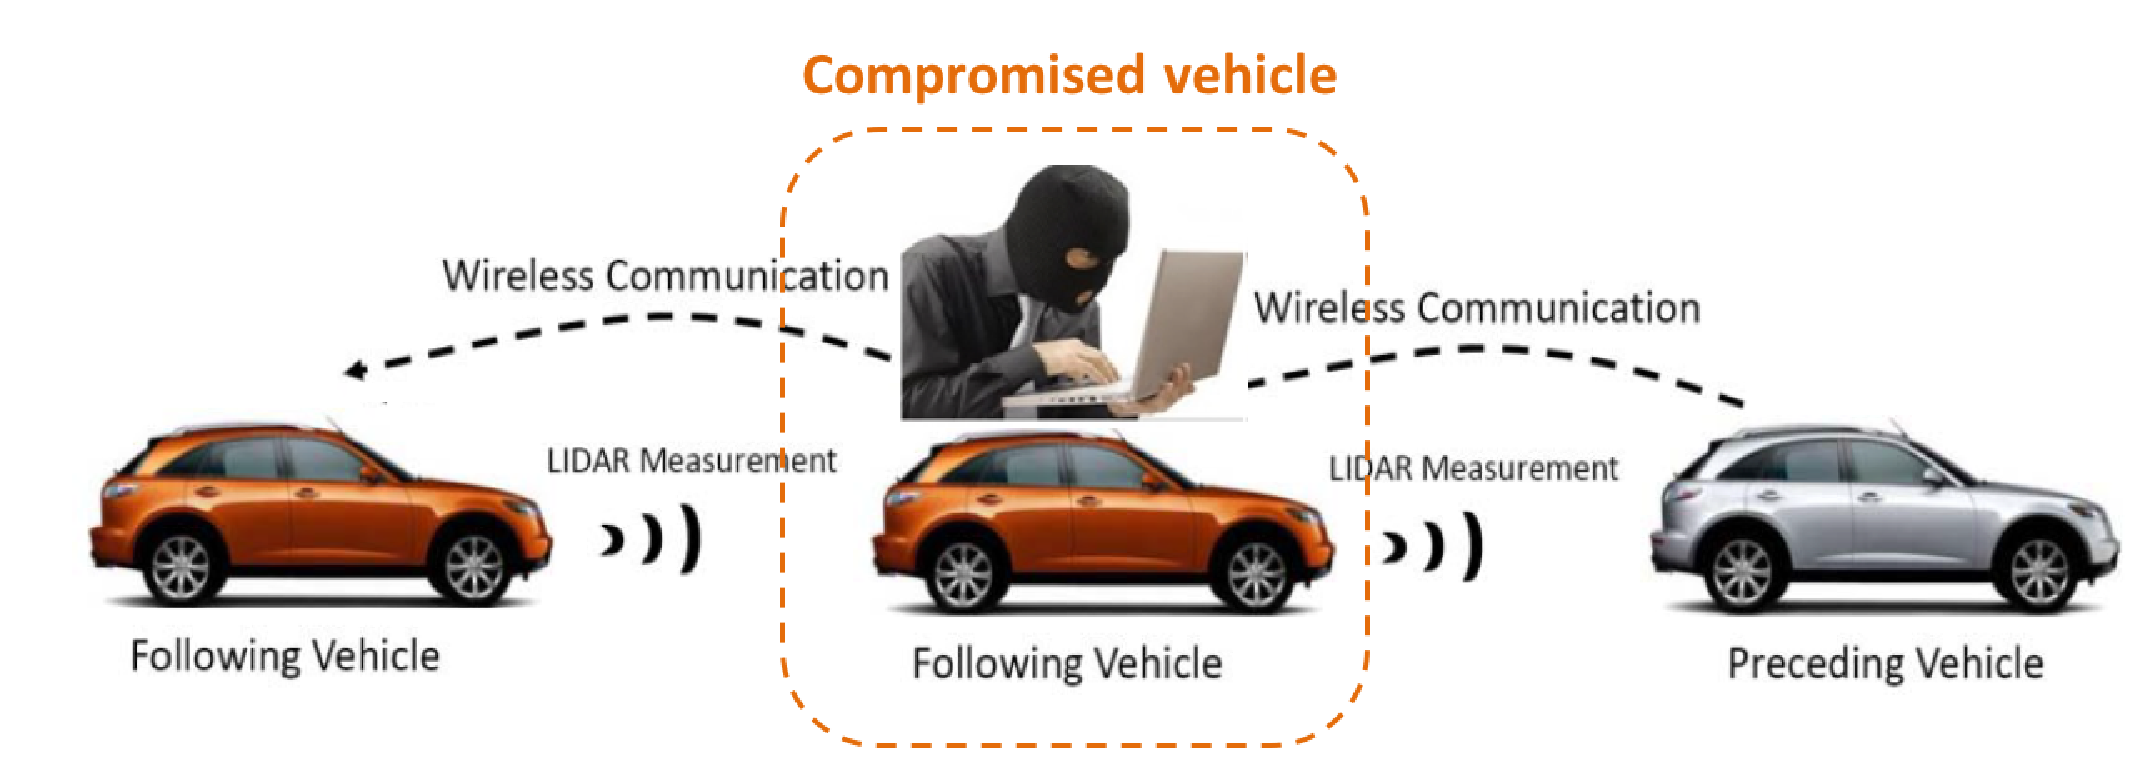
\includegraphics[width=3.8in]{GT.eps}
     }
 \end{picture}
\begin{itemize}
\item Game Theory : Attack Resilient Countermeasure
\begin{itemize}
\small 
\item One or more than one of the subsystems in distributed networked CPS are malicious
\item Malicious components trying to maximize the global cost function
\item The rest of the group want to minimize the cost function
\item Win- lose Game theory
\item Control countermeasure is performed based on game theory
\normalsize
 \end{itemize}
 \end{itemize}
\end{slide}


\section[tocsection=true,slide=false]{VI. Experimental Setup}
\begin{slide}{Experimental Setup}
\begin{picture}(0,0)
   \put(35,-215){
     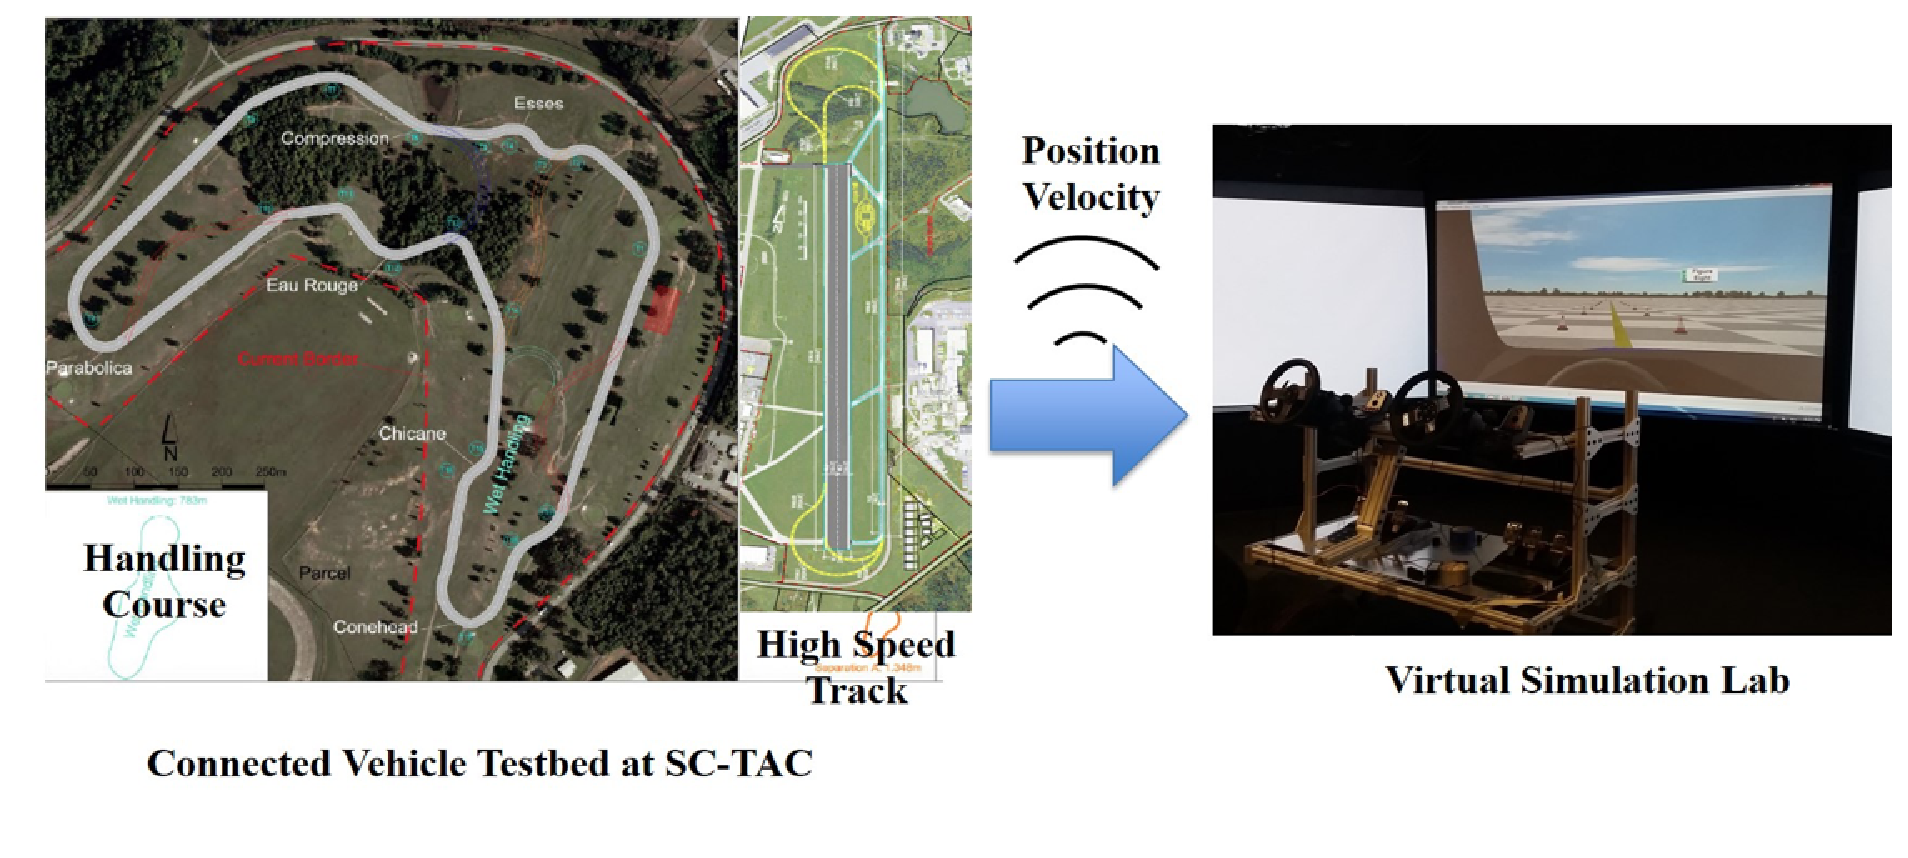
\includegraphics[width=3in]{expmt.eps}
     }
 \end{picture}
\begin{itemize}
\item Experimental testing and validation has 2 main components 
\begin{itemize}
\small 
\item CV testbed located at South Carolina Technology 
\begin{itemize}
\small 
\item More than 2.5-miles of straightaway test track, 
\item 2.5-mile interstate-grade test track  (expandable up to 17.5 miles) DSRC-based communication network for V2V and V2I 

\normalsize
 \end{itemize}
\item  Aviation Center (SC-TAC); a CV virtual/simulation lab at CU-ICAR

\normalsize
 \end{itemize}
 \end{itemize}
\end{slide}


\begin{slide}{}\tiny
%\begin{equation}
%L_i(t) =\underbrace{\omega_1\frac{Fuel}{v_i(t)}}_{\tiny{Fuel consumption}} + \underbrace{\omega_2R_{error}^2}_{\tiny{Distance to the front car}} + \underbrace{\omega_3(v_i(t+1)-v_{i-1}(t+1))^2}_{\tiny{velocity  difference between the (i+1)th car and the ith car}} + \underbrace{\omega_4 \hat{a}_i(t)^2}_{\tiny{minimize the acceleration}} + \underbrace{\omega_5(v_{i}(t+1)-v_{i+1}(t+1))^2}_{\tiny{velocity  difference between the ith car and the (i+1)th car}}
%\label{cost_middle}
%\end{equation}
\begin{equation}
L_i(t) = w_1 \int_{\Delta t} \frac{\textrm{Fuel}}{v_i(t)} + w_2 R_{\textrm{error}}^2 + w_6 R_{\textrm{error}}^2 + 
\end{equation}
\end{slide}

%\section[tocsection=true,slide=false]{II. RELATED WORK}
%\begin{slide}{Related Work}
%  \begin{itemize}
%  \item Malware uses traffic camouflaging to hide network traffic.
%   	\begin{itemize}
%  	\small 
%  	\item Spyware Taidoor (2008): Yahoo blog $\rightarrow$ C\&C server
%  	\item ChewBacca and Zeus (2014): Tor
%  	\item Pushdo malware (2013): include educational institutions into C\&C domains
%  	\item Morto Trojan (2015): send false DNS requests to a DNS server (C\&C server)
%  	 \end{itemize} 
%  \end{itemize}
%\end{slide}
%\begin{slide}{Related Work}
% \begin{itemize}
%  \item Traffic camouflage can also be used to evade surveillance and censorship: Tor, Obfsproxy, Pluggable Transport
%   	\begin{itemize}
%  	\small 
%  	\item ScrambleSuit: polymorphic network protocol against active probing and protocol fingerprinting
%  	\item SkypeMorph: reshape Tor packets to resemble Skype calls
%  	\item StegoTorus: packet chopping and steganography
%  	\item Format-transforming encryption (FTE): transform Tor traffic to match a pre-defined regular expression
%  	 \end{itemize} 
%  \end{itemize}
%\end{slide}
%
%\section[tocsection=true,slide=false]{III. BACKGROUND}
%\begin{slide}{A. Malware Traffic Detection}
%  \begin{itemize}
%  \item DPI
%  	\begin{itemize}
%  	\small
%  	\item Known signatures
%  	\item Easily foiled by encryption \\
%  	and obfuscation
%  	\normalsize
%  	\end{itemize}
%  \item Anomaly Detection
%  	\begin{itemize}
%  	\small
%  	\item High false positives (FPs)
%  	\normalsize
%  	\end{itemize}
%  \item Traffic Analysis
%  	\begin{itemize}
%  	\small
%  	\item Timing, packet size, power consumption, electromagnetic radiation, etc.
%  	\item Examples (Tor, Zbot)
%  	\normalsize
%  	\end{itemize}
%  \end{itemize}
%  \begin{picture}(0,0)
%    \put(150,90){
%      \includegraphics[width=5cm,height=2.5cm]{dpi.eps}
%      }
%  \end{picture}
%\end{slide}
%\begin{slide}{B. Format-transforming encryption}
%  \begin{itemize}
%  \item Extend conventional symmetric encryption by formatting the ciphertext
%  \item Transform a string to match a pre-defined regular expression (regex)
%   \item[]
%    \item[]
%     \item[]
%      \item[]
%       \item[]
%  \begin{picture}(0,0)
%    \put(0,0){
%      \includegraphics[width=9cm,height=2cm]{fte-general.eps}
%      }
%  \end{picture}  
%    \begin{itemize}
%  	\small 
%  	\item Input: a string, target regex, parameter (fixed\_slice)
%  	\item Output: transformed string that matches the target regex
%  	\end{itemize}
% \item For example
%    \begin{itemize}
%  	\small 
%  	\item Input: 'helloworld', '$\wedge(a|b)+\$$', fixed\_slice=512
%  	\item Output: 'aaaaaaaabababaab...bababbabaaababab' (length = 512)
%  	\end{itemize}
%  \end{itemize}
%\end{slide}
%\begin{slide}{B. FTE}
%FTE Procedures
%  \begin{picture}(0,0)
%    \put(-90,-165){
%      \includegraphics[width=11cm,height=5cm]{fte-detail.eps}
%      }
%  \end{picture}  
%\end{slide}
%\begin{slide}{B. FTE}
%How to \textcolor{red}{rank/unrank} a regular language?
%  \begin{picture}(0,0)
%    \put(-190,-185){
%      \includegraphics[width=10cm,height=6cm]{rank.eps}
%      }
%  \end{picture}  
%\end{slide}
%\begin{slide}{C. Zeus Botnet}
%  \begin{itemize}
%  \item A botnet is a collection of compromised computers on the Internet
%  \item Compromised computers are usually controlled by a centralized command and control (C\&C) server
%  \item Malicious actions
%  	\begin{itemize}\small
%  	\item Spam
%  	\item Distributed DoS attack
%  	\item Stealing login credentials \\
%  	or personal information\normalsize
%  	\end{itemize}
%  \end{itemize}
%  \begin{picture}(0,0)
%    \put(180,-10){
%      \includegraphics[width=4cm,height=3cm]{botnet.eps}
%      }
%  \end{picture}
%\end{slide}
%\begin{slide}{C. Zeus Botnet}
%  \begin{itemize}
%  \item Zbot uses key-logging techniques to steal sensitive data for online accounts on windows machines
%  \item By July 2009, Zbot was estimated to include millions of compromised computers (around 3.6 million in the United States).
%  \item No.1 of America's 10 most wanted botnets\textsuperscript{[1]}
%  \item[]
%   \item[]
%    \item[]
%     \item[]
%      \item[]
%       \item[]
%       	\item[]
%       	 \item[]
%  \end{itemize}
%  \begin{picture}(0,0)
%    \put(80,30){
%      \includegraphics[width=5cm,height=3cm]{wordbot.eps}
%      }
%  \end{picture}
%  \tiny
%  [1] http://www.computerworld.com/s/article/9135861/America\_s\_10\_most\_wanted\_botnets
%  \normalsize
%\end{slide}
%\begin{slide}{C. Zeus Botnet}
%  \begin{itemize}
%  \item Zbot uses key-logging techniques to steal sensitive data for online accounts on windows machines
%  \item By July 2009, Zbot was estimated to include millions of compromised computers (around 3.6 million in the United States).
%  \item No.1 of America's 10 most wanted botnets\textsuperscript{[1]}
%  \item[]
%   \item[]
%    \item[]
%     \item[]
%      \item[]
%       \item[]
%        \item[]
%         \item[]
%  \end{itemize}
%  \begin{picture}(0,0)
%    \put(80,30){
%      \includegraphics[width=5cm,height=3cm]{wordbot.eps}
%      }
%  \end{picture}
%  \begin{picture}(0,0)
%    \put(60,20){
%      \includegraphics[width=6cm,height=6cm]{crime2.eps}
%      }
%  \end{picture}
%  \tiny
%  [1] http://www.computerworld.com/s/article/9135861/America\_s\_10\_most\_wanted\_botnets
%  \normalsize
%\end{slide}
%\begin{slide}{C. Zeus Botnet}
%  \begin{itemize}
%  \item Zbot uses key-logging techniques to steal sensitive data for online accounts on windows machines
%  \item By July 2009, Zbot was estimated to include millions of compromised computers (around 3.6 million in the United States).
%  \item No.1 of America's 10 most wanted botnets\textsuperscript{[1]}
%  \item[]
%   \item[]
%    \item[]
%     \item[]
%      \item[]
%       \item[]
%        \item[]
%  \end{itemize}
%  \begin{picture}(0,0)
%    \put(80,30){
%      \includegraphics[width=5cm,height=3cm]{wordbot.eps}
%      }
%  \end{picture}
%  \begin{picture}(0,0)
%    \put(60,20){
%      \includegraphics[width=6cm,height=6cm]{crime2.eps}
%      }
%  \end{picture}
%  \begin{picture}(0,0)
%    \put(30,80){
%      \includegraphics[width=8cm,height=1cm,]{crime1.eps}
%      }
%  \end{picture}
%  \tiny
%  [1] http://www.computerworld.com/s/article/9135861/America\_s\_10\_most\_wanted\_botnets
%  \normalsize
%\end{slide}\begin{slide}{C. Zeus Botnet}
%  \begin{itemize}
%  \item Zbot uses key-logging techniques to steal sensitive data for online accounts on windows machines
%  \item By July 2009, Zbot was estimated to include millions of compromised computers (around 3.6 million in the United States).
%  \item No.1 of America's 10 most wanted botnets\textsuperscript{[1]}
%  \item[]
%   \item[]
%    \item[]
%     \item[]
%      \item[]
%       \item[]
%        \item[]
%  \end{itemize}
%  \begin{picture}(0,0)
%    \put(80,30){
%      \includegraphics[width=5cm,height=3cm]{wordbot.eps}
%      }
%  \end{picture}
%  \begin{picture}(0,0)
%    \put(60,20){
%      \includegraphics[width=6cm,height=6cm]{crime2.eps}
%      }
%  \end{picture}
%  \begin{picture}(0,0)
%    \put(30,80){
%      \includegraphics[width=8cm,height=1cm,]{crime1.eps}
%      }
%  \end{picture}
%  \begin{picture}(0,0)
%    \put(30,10){
%      \includegraphics[width=8cm,height=4cm,]{crime3.eps}
%      }
%  \end{picture}
%  \tiny
%  [1] http://www.computerworld.com/s/article/9135861/America\_s\_10\_most\_wanted\_botnets
%  \normalsize
%\end{slide}
%\begin{slide}{D. Smart Grid Communications}
%  \begin{itemize}
%  \item Phasor Measurement Unit (PMU)
%  	\begin{itemize}
%  	\small
%  	\item Send measurements to \\
%  	phasor data concentrators (PDCs).
%  	\item Measurements include voltage,\\
%  	line currents, and bus frequencies.
%  	\item Synchrophasor protocol\\
%  	(TCP based)
%  	\item Currently in clear text...
%  	\normalsize
%  	\end{itemize}
%  \item OpenPDC is an open source software.
%  \end{itemize}
%  \begin{picture}(0,0)
%    \put(180,0){
%      \includegraphics[width=4.5cm,height=5cm]{pmu.eps}
%      }
%  \end{picture}
%\end{slide}
%
%\section[tocsection=true,slide=false]{IV. METHOD}
%\begin{slide}{The Proposed Traffic Camouflage Approach}
%  \begin{picture}(0,0)
%    \put(0,-90){
%      \includegraphics[width=10cm,height=3.5cm]{before.eps}
%      }
%  \end{picture}
%    \begin{picture}(0,0)
%    \put(0,-210){
%      \includegraphics[width=10cm,height=3.5cm]{after.eps}
%      }
%  \end{picture}
%\end{slide}
%
%\begin{slide}{A. Improved FTE}
%\begin{itemize}
%\item[]
%\item Goal: transform Zbot traffic (TCP+HTTP) to PMU traffic (synchrophasor protocol) offline
%\item[]
%\item Steps:
%\begin{enumerate}
%\item Capture Zbot traffic as PCAP files
%\item Take all payloads of Zbot packets as input string to FTE
%\item Transform the input string into an intermediate output string that matches regex '$\wedge[0-9a-f]+\$$'
%\item \textcolor{blue}{Map} the intermediate output string to PMU traffic
%\item Send out PMU traffic as payloads between tcp client and server
%\end{enumerate}
%\end{itemize}
%\end{slide}
%
%\begin{slide}{A. Improved FTE}
%\begin{itemize}
%\item The mapping technique: \\
%\vspace{1cm}
%\fbox{
%    \parbox{0.8\textwidth}{\centering
%intermediate output string \\
%(each character in the string is 0-9,a-f)
%    }
%}
%\\
%\vspace{0.5cm}
%\centering$\Downarrow$ 	
%\vspace{0.5cm}
%\\
%\fbox{
%    \parbox{0.5\textwidth}{\centering
%PMU traffic
%    }
%}
%\end{itemize}
%\end{slide}
%
%\begin{slide}{A. Improved FTE}
%\begin{itemize}
%\item The mapping requires some information (a \textcolor{blue}{dictionary}) about PMU traffic.
%\item We collected 108.9MB PMU traffic and looked into the packet payload (application layer, length = 284 bytes).
%\item We gathered all observed values for each field in PMU, and built a dictionary for each field (14 dictionaries totally).
%\item For each dictionary, we divided it into 16 groups.
%\item One character will be mapped to value in one field.
%\item The mapping technique: Convert output string to chunks (length = 284 bytes)
%\end{itemize}
%\end{slide}
%
%\begin{slide}{A. Improved FTE}
%\begin{itemize}
%\item[]
%\item For example, the output \\
%string is ‘a10b5d7...’. \\
%(hexadecimal string)
%\item[]
%\item[]
%\item For the first character ‘a’:\\
%'a' (hex) $\rightarrow$ '10' (dec)\\
%Index=1 $\rightarrow$ dict 1\\
%Look up a random value \\from group 10 in dict 1\\ (SOC time stamp(UTC))
%\end{itemize}
%  \begin{picture}(0,0)
%    \put(145,-20){
%      %\includegraphics[width=5.5cm,height=7cm]{1_3.eps}
%      \includegraphics[width=5.5cm,height=7cm]{field.eps}
%      }
%  \end{picture}
%\end{slide}
%
%\begin{slide}{A. Improved FTE}
%\begin{itemize}
%\item \textcolor{blue}{Advantages} over original FTE:
%\begin{itemize}
%\small
%\item Input regex is straightforward $\rightarrow$ no need to make up complex regex
%\item No complex regex $\rightarrow$ automated process
%\item Use observed PMU traffic $\rightarrow$ closer than outputs by original FTE
%\item The throughput is increased
%\end{itemize}
%\end{itemize}
%\end{slide}
%
%\begin{slide}{B. Timing Side-Channel Massage (SCM)}
%\begin{itemize}
%\item Timing SCM modifies inter-packet delays to match the target protocol to evade side-channel analysis. 
%\end{itemize}
%  \begin{picture}(0,0)
%    \put(0,-150){
%      %\includegraphics[width=5.5cm,height=7cm]{1_3.eps}
%      \includegraphics[height=5.5cm]{1.eps}
%      }
%  \end{picture}
%\end{slide}
%
%\section[tocsection=true,slide=false]{V. EXPERIMENT}
%\begin{slide}{A. Traffic Collection}
%\begin{itemize}
%\item A Zeus C\&C server and\\
% a Zeus bot are set up \\
% in the lab on two \\
% Windows XP virtual\\
%  machines. 
%\item[]
%\item[]
%\item Network traffic between\\
% PMU and PDC are collected\\
%  with Wireshark on the same \\
%  machine (windows 7 OS) \\
%  running openPDC software. 
%\end{itemize}
%  \begin{picture}(0,0)
%    \put(150,120){
%      %\includegraphics[width=5.5cm,height=7cm]{1_3.eps}
%      \includegraphics[width=5.5cm]{2_1.eps}
%      }
%    \put(150,30){
%      %\includegraphics[width=5.5cm,height=7cm]{1_3.eps}
%      \includegraphics[width=5.5cm]{2_2.eps}
%      }
%  \end{picture}
%        
%\end{slide}
%
%
%\begin{slide}{B. Experiment Setup}
%\begin{itemize}
%\item[]
%\item[]
%\item[]
%\item[]
%\item[]
%\item[]
%\item The implementation includes a client-side program (counterfeit PMU program) deployed on the bot and a decoder integrated as a front end of C\&C server. The client-side program takes the Zbot data stream as input, processes it with FTE then SCM. It then sends the false PMU data over the network. When the data arrives at the server side, it is decoded by the FTE decoder and forwarded the to C\&C server. 
%\end{itemize}
%  \begin{picture}(0,0)
%    \put(0,150){
%      %\includegraphics[width=5.5cm,height=7cm]{1_3.eps}
%      \includegraphics[width=300pt]{3.eps}
%      }
%  \end{picture}
%\end{slide}
%
%
%\begin{slide}{C. Experiment, Results and Analysis  }
%  \begin{picture}(0,0)
%    \put(20,-90){
%      %\includegraphics[width=5.5cm,height=7cm]{1_3.eps}
%      \includegraphics[width=260pt]{4_1.eps}
%      }
%    \put(20,-200){
%      %\includegraphics[width=5.5cm,height=7cm]{1_3.eps}
%      \includegraphics[width=260pt]{4_2.eps}
%      }
%  \end{picture}
%        
%\end{slide}
%
%
%\begin{slide}{C. Experiment, Results and Analysis  }
%  \begin{picture}(0,0)
%    \put(-10,-160){
%      %\includegraphics[width=5.5cm,height=7cm]{1_3.eps}
%      \includegraphics[width=320pt]{5.eps}
%      }
%  \end{picture}
%        
%\end{slide}
%
%
%\begin{slide}{C. Experiment, Results and Analysis  }
%  \begin{picture}(0,0)
%    \put(-10,-80){
%      %\includegraphics[width=5.5cm,height=7cm]{1_3.eps}
%      \includegraphics[width=320pt]{6.eps}
%      }
%  \end{picture}
%   \begin{itemize}
%\item[]
%\item[]
%\item[]
%\item[]
%\item[]
%\item[]
%\item[]
%\item A communication channel is built between the counterfeit PMU and software OpenPDC. All false PMU traffic is accepted by OpenPDC. This shows that the proposed method is capable of producing false PMU data stream close to real PMU. 
%\end{itemize}
%
%\end{slide}
%
%
%\section[tocsection=true,slide=false]{VI. CONCLUSION}
%\begin{slide}{CONCLUSION AND FUTURE WORK}
%   \begin{itemize}
%\item One protocol is transformed into another to disguise the original traffic and deceive existing network traffic detection approaches, including side-channel analysis. 
%\item Zbot C\&C traffic is transformed to PMU data stream. The experiment shows that the syntax of the counterfeit PMU packet is consistent with real PMU traffic. The proposed method is also resistant to timing side-channel analysis. False PMU packets are accepted by OpenPDC without any errors. Other target protocols can easily be used. 
%\end{itemize}
%\end{slide}
%
%\begin{slide}{CONCLUSION AND FUTURE WORK}
%   \begin{itemize}
%\item The proposed traffic camouflage counter- countermeasure is not perfect. Future study includes:
%   \begin{itemize}
%\item On-line implementation. 
%\item The throughput can be increased by determining the optimal number of character positions used to represent a packet field. 
%\item Methods of selecting appropriate target protocols are needed. 
%\item The ultimate goal of this study is to make anti-virus community aware of this new way of hiding malware traffic and therefore effective countermeasures are needed. 
%\end{itemize}
%\end{itemize}
%\end{slide}
%
%
%\begin{slide}{Questions?}
%   \begin{itemize}
%\item[]
%\item[]
%\item[]
%\item[]
%\item 				Questions?
%\end{itemize}
%
%\end{slide}


\end{document}